\subsection*{Partie A}

\begin{enumerate}
\item \begin{minipage}[t]{0.4\linewidth}
La situation peut être représentée par l'arbre pondéré ci-contre :
\end{minipage}
\hfill
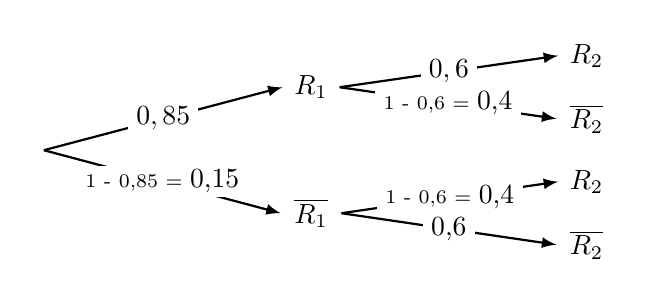
\begin{tikzpicture}[xscale=1,yscale=1,baseline={(R.base)}]
		
		\tikzstyle{fleche}=[->,>=latex,thick]
		\tikzstyle{noeud}=[fill=white,circle,inner sep=2pt]
		\tikzstyle{feuille}=[fill=white,circle,inner sep=2pt]
		\tikzstyle{etiquette}=[pos=0.5,fill=white, inner xsep=3pt, inner ysep=1.5pt]
		
		\def\DistanceInterNiveaux{3.5}
		\def\DistanceInterFeuilles{0.8}
		
		\def\NiveauA{(0)*\DistanceInterNiveaux}
		\def\NiveauB{(1)*\DistanceInterNiveaux}
		\def\NiveauC{(2)*\DistanceInterNiveaux}
		\def\InterFeuilles{(-1)*\DistanceInterFeuilles}
		
		\node[noeud] (R) at ({\NiveauA},{(1.5)*\InterFeuilles}) {};
		\node[noeud] (Ra) at ({\NiveauB},{(0.5)*\InterFeuilles}) {$R_1$};
		\node[feuille] (Raa) at ({\NiveauC},{(0)*\InterFeuilles}) {$R_2$};
		\node[feuille] (Rab) at ({\NiveauC},{(1)*\InterFeuilles}) {$\overline{R_2}$};
		\node[noeud] (Rb) at ({\NiveauB},{(2.5)*\InterFeuilles}) {$\overline{R_1}$};
		\node[feuille] (Rba) at ({\NiveauC},{(2)*\InterFeuilles}) {$R_2$};
		\node[feuille] (Rbb) at ({\NiveauC},{(3)*\InterFeuilles}) {$\overline{R_2}$};
		
		\draw[fleche] (R.east)--(Ra.west) node[etiquette] {$0,85$};
		\draw[fleche] (Ra.east)--(Raa.west) node[etiquette] {$0,6$};
		\draw[fleche] (Ra.east)--(Rab.west) node[etiquette] {{\red {\scriptsize 1 - 0,6 = }0,4}};
		\draw[fleche] (R.east)--(Rb.west) node[etiquette] {{\red {\scriptsize 1 - 0,85 = }0,15}};
		\draw[fleche] (Rb.east)--(Rba.west) node[etiquette] {{\red {\scriptsize 1 - 0,6 = }0,4}};
		\draw[fleche] (Rb.east)--(Rbb.west) node[etiquette] {0,6};
\end{tikzpicture}

	\item Les évènement $R_1$ et $\overline{R_1}$ partitionnent l'univers, donc, d'après la loi des probabilités totales, on a :

$P(R_2) = P\big(R_2 \cap R_1\big) + P\big(R_2 \cap \overline{R_1}\big) = 0,85 \times 0,6 + 0,15 \times 0,4 = 0,57$.

Ceci confirme que la probabilité de l'évènement $R_{2}$ est égale à 0,57.

	\item Sachant que le joueur a réussi le deuxième service, la probabilité qu'il ait raté le premier est la probabilité conditionnelle : \quad $P_{R_2} \big(\overline{R_1}\big)$.

D'après la définition :\quad $P_{R_2} \big(\overline{R_1}\big) = \dfrac{P\big(R_2 \cap \overline{R_1}\big)}{P(R_2)} = \dfrac{0,15 \times 0,4}{0,57} = \dfrac{0,06}{0,57} = \dfrac{6}{57} = \dfrac{2}{19}$.

(puisqu'il n'y a pas de consigne d'arrondi dans l'énoncé, \emph{a priori}, c'est la valeur exacte, fractionnaire, qui est attendue).

	\item \begin{enumerate}
		\item Voici le tableau donnant  la loi de probabilité de $Z$.

		\begin{tabularx}{\linewidth}{|c|*{3}{>{\centering \arraybackslash}X|}} \hline
			$z_i$ & 0&1&2\\ \hline
			évènement & $\overline{R_1} \cap \overline{R_2}$& \Big($\overline{R_1} \cap R_2\Big) \cup \Big(R_1 \cap \overline{R_2}\Big)$& $R_1 \cap R_2$\\ \hline
			$P(Z = z_i)$& {\scriptsize $0,15 \times 0,6 =$} 0,09&{\scriptsize $0,15 \times 0,4 +0,85 \times 0,4=$} {\scriptsize $0,06 +0,34 =$} 0,4&{\scriptsize $0,85 \times 0,6 = $} 0,51 \\ \hline
		\end{tabularx}

		\item L'espérance mathématique $\mathrm{E}(Z)$ est donc :

		$E(Z) = 0,09 \times 0 + 0,4 \times 1 + 0,51 \times 2 = 1,42$.

Ce résultat, dans le contexte de l'exercice, signifie que, dans ces conditions, le nombre moyen de services réussis sur les deux premiers services de la séance d'entraînement est de 1,42.

(Ici, le nombre 1,42 n'a pas a être arrondi à l'entier, car il ne représente pas un nombre réel ou réaliste de services réussis, mais une \emph{moyenne} théorique, établie sur les deux premiers services d'un grand nombre d'entraînements réalisés dans les mêmes conditions).
	\end{enumerate}
\end{enumerate}

\subsection*{Partie B}

\begin{enumerate}
	\item \begin{enumerate}
		\item D'après l'énoncé, on a les probabilités conditionnelles suivantes :

		\begin{itemize}[label=$\bullet$]
			\item $P_{R_{n}}\left(R_{n + 1}\right) = 0,6$ : c'est la situation \og si le joueur réussit un service (ici, le service $n$) alors la probabilité qu'il réussise le suivant (ici, le service $(n+1)$) est égale à 0,6\fg{}.
			\item  $P_{\overline{R_{n}}}\left(\overline{R_{n + 1}}\right) = 0,6$. Là, c'est la situation \og si le joueur ne réussit pas un service (ici, le service $n$) alors la probabilité qu'il ne réussisse pas le suivant (ici, le service $(n+1)$) est égale à 0,6\fg{}.
		\end{itemize}

		\item \begin{minipage}[t]{0.4\linewidth}
		On peut visualiser la situation par l'arbre pondéré ci-contre : \end{minipage}
	\hfill
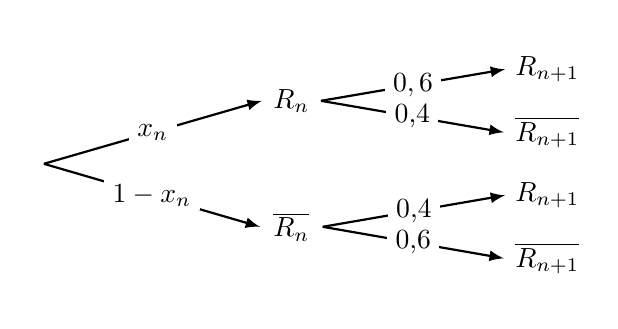
\begin{tikzpicture}[xscale=1,yscale=1,baseline={(R.base)}]

\tikzstyle{fleche}=[->,>=latex,thick]
\tikzstyle{noeud}=[fill=white,circle,inner sep=2pt]
\tikzstyle{feuille}=[fill=white,circle,inner sep=2pt]
\tikzstyle{etiquette}=[pos=0.5,fill=white, inner xsep=3pt, inner ysep=1.5pt]

\def\DistanceInterNiveaux{3.25}
\def\DistanceInterFeuilles{0.8}

\def\NiveauA{(0)*\DistanceInterNiveaux}
\def\NiveauB{(1)*\DistanceInterNiveaux}
\def\NiveauC{(2)*\DistanceInterNiveaux}
\def\InterFeuilles{(-1)*\DistanceInterFeuilles}

\node[noeud] (R) at ({\NiveauA},{(1.5)*\InterFeuilles}) {};
\node[noeud] (Ra) at ({\NiveauB},{(0.5)*\InterFeuilles}) {$R_n$};
\node[feuille] (Raa) at ({\NiveauC},{(0)*\InterFeuilles}) {$R_{n+1}$};
\node[feuille] (Rab) at ({\NiveauC},{(1)*\InterFeuilles}) {$\overline{R_{n+1}}$};
\node[noeud] (Rb) at ({\NiveauB},{(2.5)*\InterFeuilles}) {$\overline{R_n}$};
\node[feuille] (Rba) at ({\NiveauC},{(2)*\InterFeuilles}) {$R_{n+1}$};
\node[feuille] (Rbb) at ({\NiveauC},{(3)*\InterFeuilles}) {$\overline{R_{n+1}}$};

\draw[fleche] (R.east)--(Ra.west) node[etiquette] {$x_n$};
\draw[fleche] (Ra.east)--(Raa.west) node[etiquette] {$0,6$};
\draw[fleche] (Ra.east)--(Rab.west) node[etiquette] {0,4};
\draw[fleche] (R.east)--(Rb.west) node[etiquette] {$1 - x_n$};
\draw[fleche] (Rb.east)--(Rba.west) node[etiquette] {0,4};
\draw[fleche] (Rb.east)--(Rbb.west) node[etiquette] {0,6};
\end{tikzpicture}

$R_n$ et $\overline{R_n}$ partitionnant l'univers, d'après la loi des probabilités totales, on a :

$\begin{aligned}[t] x_{n+1} &= P(R_{n+1}) \\
&= P\big(R_{n+1} \cap R_n\big)P\big(R_{n+1} \cap \overline{R_n}\big)\\
&= x_n \times 0,6 + (1 - x_n)\times 0,4 \\
&= 0,6 x_n + 0,4 - 0,4x_n \\
&= 0,2x_n + 0,4.\end{aligned}$

On a bien établi la relation de récurrence attendue pour la suite $(x_n)$.
	\end{enumerate}

	\item \begin{enumerate}
		\item Puisque l'on a, pour tout entier naturel non nul $u_n = x_n - 0,5$, c'est équivalent à dire que l'on a $u_n + 0,5 = x_n$.

		Cherchons à établir la relation de récurrence de la suite $(u_n)$. Soit $n$ un entier naturel non nul :

$\begin{aligned}[t] u_{n+1} &= x_{n+1} - 0,5 &\text{d'après la définition de la suite }(u_n)\\
&=\big(0,2 x_n + 0,4\big) -0,5&\text{d'après la relation de récurrence de }(x_n) \\
&&\text{ (voir \textbf{B 1. b.})}\\
&=0,2 \big(u_n + 0,5\big) + 0,4 - 0,5&\text{d'après la définition de la suite }(u_n)\\
&=0,2u_n + 0,2\times 0,5 - 0,1\\
&=0,2u_n + 0,1 - 0,1\\
&=0,2u_n\\ \end{aligned}$

Cette relation de récurrence est celle d'une suite géométrique, de raison $q= 0,2$ et de premier terme $u_1 = x_1 - 0,5 = 0,85 - 0,5 = 0,35$.

	\item Puisque l'on sait que $(u_n)$ est géométrique, on a :

$\forall n \in \N^*,\quad u_n = u_1 \times q^{n-1} = 0,35 \times 0,2^{n-1}$.

Et comme, pour tout $n$ naturel non nul $u_n + 0,5 = x_n$ :\quad $x_n = 0,5 + 0,35 \times 0,2^{n-1}$

Comme on a $0 < 0,2 < 1$, on en déduit :\quad$\lim\limits_{n \to +\infty} u_n = 0$,

	et donc, par limite de la somme :\quad $\lim\limits_{n \to +\infty} x_n = 0,5$.


	\item Dans le contexte de l'exercice, cela signifie qu'au bout d'un grand nombre de services, la probabilité de réussir un service tend à se stabiliser aux alentours de 0,5, ou bien encore qu'au bout d'un grand nombre de services, le joueur aura tendance à réussir un service sur 2.
\end{enumerate}
\end{enumerate}
